\documentclass[border=10pt]{standalone}

\usepackage{tikz}
\usepackage{tikzsymbols}
\usetikzlibrary{calc,patterns,shapes.geometric}

\def\centerarc[#1](#2)(#3:#4:#5){\draw[#1] ($(#2)+({#5*cos(#3)},{#5*sin(#3)})$) arc (#3:#4:#5);}

\begin{document}
	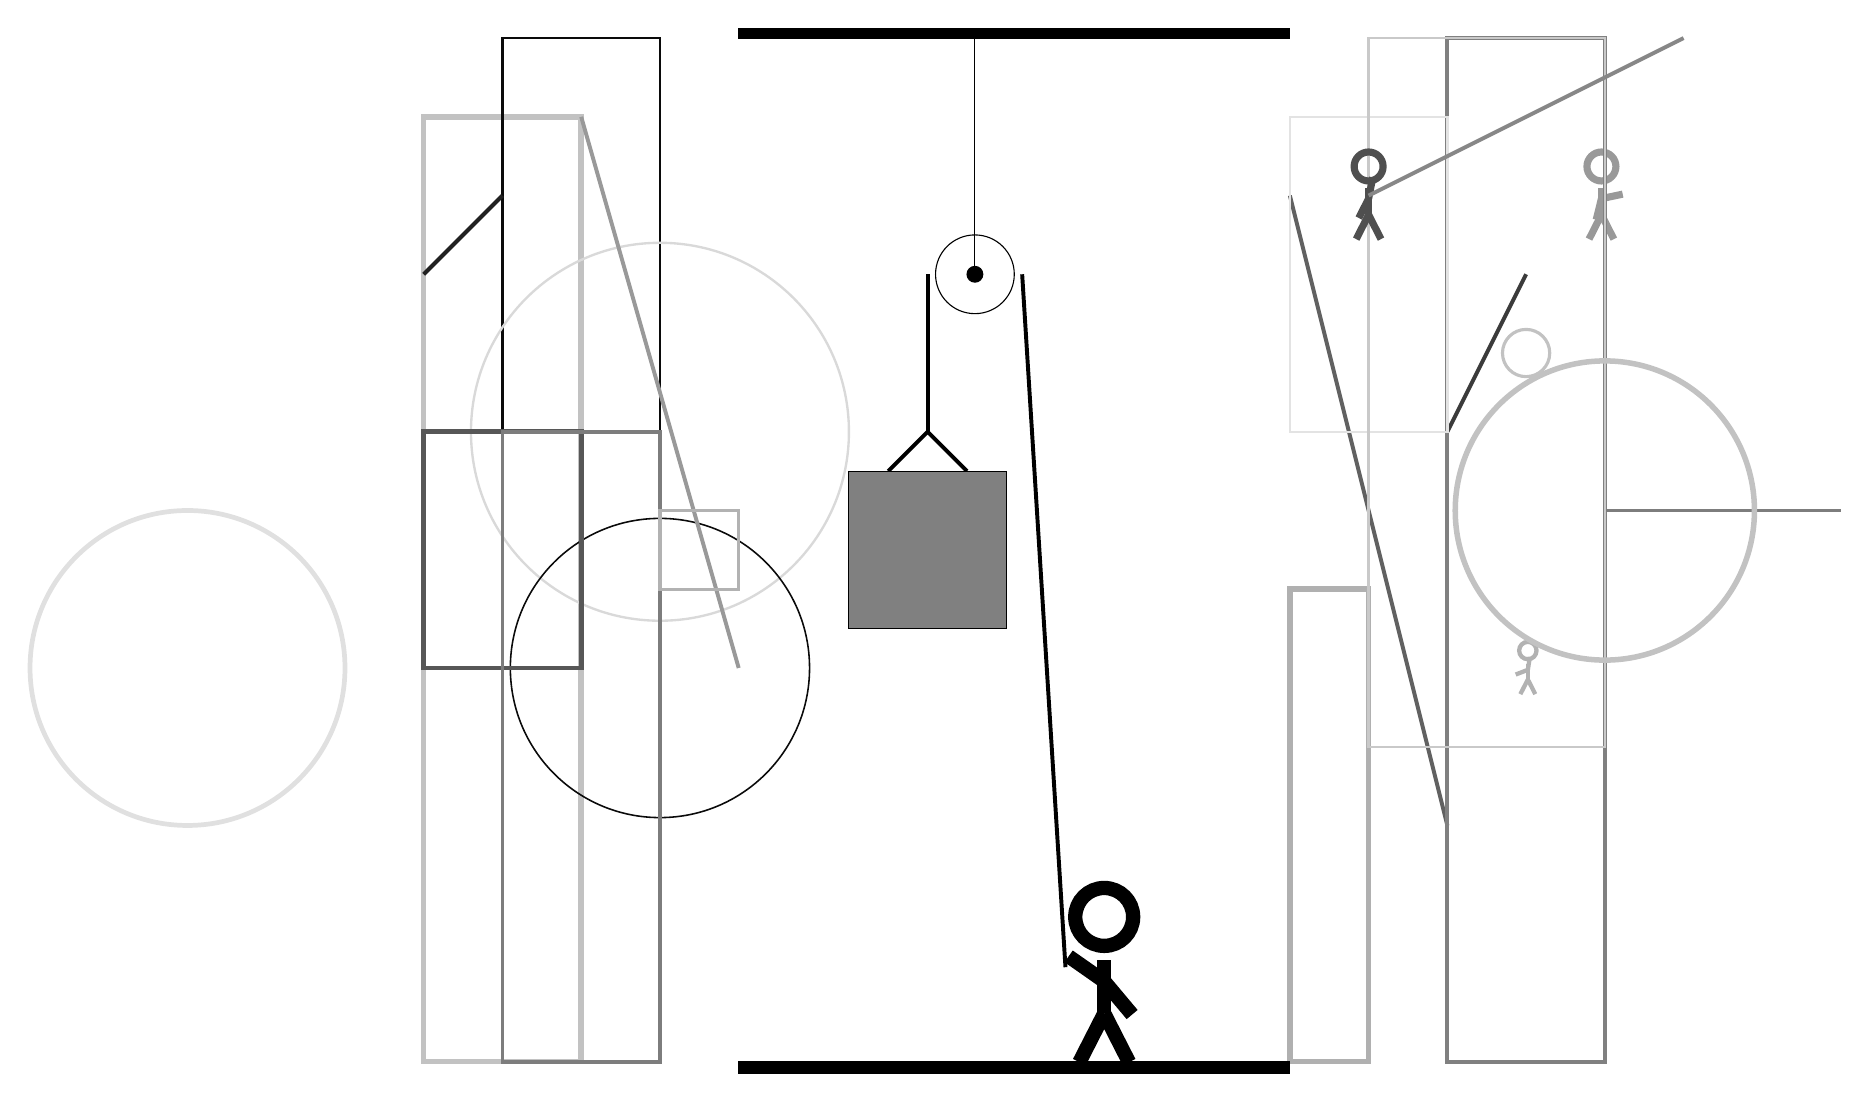
\begin{tikzpicture}
		%%%%% START %%%%%
		
		\draw[fill=black] (-2, 10) rectangle (5, 10.125);
		
		\draw (1, 7) circle (0.5);
		\draw[fill=black] (1, 7) circle (0.1);
		\draw (1, 10) -- (1, 7);
		
		\draw[line width=0.5mm] (-0.1, 4.5) -- (0.4, 5.0) -- (0.9, 4.5);
		\draw[fill=black!50] (-0.6, 4.5) rectangle (1.4, 2.5);
		
		\draw[line width=0.4mm, color=black!20] (6, 7) rectangle (6, 8);
		
		\node[line width=0.6mm, color=black!30] at (8, 2) {\Strichmaxerl[3][21][81]};
		\draw[line width=0.7mm, color=black!24] (-4, -3) rectangle (-6, 9);
		\draw[line width=0.4mm, color=black!60] (7, 6) rectangle (7, 6);
		\draw[line width=0.5mm, color=black!77](8, 7) -- (7, 5);
		
		\draw[line width=0.7mm, color=black!31] (5, 3) rectangle (6, -3);
		
		\node[line width=0.5mm, color=black!40] at (9, 8) {\Strichmaxerl[5][76][12]};
		
		\draw[line width=0.5mm, color=black!62](7, 0) -- (5, 8);
		\draw[line width=0.3mm, color=black!96] (-3, -3) rectangle (-5, 10);
		
		\draw [line width=0.3mm, color=black!15](-3, 5) circle (2.4);
		\draw[line width=0.5mm, color=black!50] (7, 10) rectangle (9, -3);
		\draw [line width=0.4mm, color=black!24](8, 6) circle (0.3);
		\draw [line width=0.6mm, color=black!12](-9, 2) circle (2.0);
		
		\draw [line width=0.2mm, color=black!96](-3, 2) circle (1.9);
		\draw[line width=0.5mm, color=black!51](9, 4) -- (12, 4);
		\draw[line width=0.3mm, color=black!11] (5, 9) rectangle (7, 5);
		
		\draw[line width=0.6mm, color=black!66] (-4, 2) rectangle (-6, 5);
		\draw[line width=0.5mm, color=black!51] (-3, 5) rectangle (-5, -3);
		\draw[line width=0.3mm, color=black!21] (6, 10) rectangle (9, 1);
		\draw [line width=0.7mm, color=black!24](9, 4) circle (1.9);
		\draw[line width=0.5mm, color=black!40](-4, 9) -- (-2, 2);
		\draw[line width=0.4mm, color=black!30] (-3, 3) rectangle (-2, 4);
		\node[line width=0.7mm, color=black!69] at (6, 8) {\Strichmaxerl[5][63][79]};
		\draw[line width=0.5mm, color=black!47](6, 8) -- (10, 10);
		\draw[line width=0.5mm, color=black!87](-6, 7) -- (-5, 8);
		
		
		\draw[line width=0.5mm] (0.4, 7) -- (0.4, 5.0);
		\centerarc[line width=0.5mm](1, 7)(0:180:0.6);
		\draw[line width=0.5mm](1.6, 7) -- (2.15, -1.8);
		
		\node at (2.6, -1.9) {\Strichmaxerl[10][-35][-50]};
		
		\draw[fill=black] (-2, -3) rectangle (5, -3.15);
		
		%%%%% END %%%%%
	\end{tikzpicture}
\end{document}